\documentclass[12pt,a4paper]{article}
\usepackage[utf8]{inputenc}
\usepackage[spanish,es-tabla]{babel}
\usepackage{geometry}
\usepackage{graphicx}
\usepackage{multirow}
\usepackage{tabularx}
\usepackage{mathptmx}
\usepackage{fancyhdr}
\usepackage{array}
\usepackage[table]{xcolor}
\usepackage{titlesec}
\usepackage{setspace}
\usepackage{microtype}
\usepackage{lastpage}
\usepackage{booktabs}
\usepackage{enumitem}
\usepackage{amsmath}
\usepackage{amsfonts}
\usepackage{amssymb}

\usepackage{float}
\usepackage{placeins}
\usepackage{tikz}
\usepackage{pgfplots}
\pgfplotsset{compat=1.17}
\usetikzlibrary{arrows.meta,positioning,shapes.geometric,calc}

\graphicspath{{images/}{../images/}{./}}

\geometry{
    top=4.7cm,
    bottom=2.5cm,
    left=2.5cm,
    right=2.5cm,
    headheight=3.9cm,
    headsep=0.4cm
}

\setstretch{1.15}
\setlength{\parindent}{0pt}
\setlength{\parskip}{0.45em}
\setlength{\tabcolsep}{4pt}

\titleformat{\section}
  {\normalfont\fontsize{12}{14.5}\bfseries}{\thesection.}{0.6em}{\uppercase}
\titlespacing*{\section}
  {0pt}{1.8ex plus 0.4ex minus 0.2ex}{0.6ex plus 0.2ex}

\titleformat{\subsection}
  {\normalfont\fontsize{11.5}{13.5}\bfseries}{\thesubsection.}{0.5em}{}
\titlespacing*{\subsection}
  {0pt}{1.4ex plus 0.3ex minus 0.1ex}{0.4ex plus 0.1ex}

\titleformat{\subsubsection}
  {\normalfont\fontsize{10.5}{12.5}\bfseries\itshape}{\thesubsubsection.}{0.4em}{}
\titlespacing*{\subsubsection}
  {0pt}{1.1ex plus 0.2ex minus 0.1ex}{0.3ex plus 0.1ex}

\newcolumntype{Y}{>{\centering\arraybackslash}X}
\newcolumntype{L}{>{\raggedright\arraybackslash}X}
\newcolumntype{C}{>{\centering\arraybackslash}X}

\definecolor{headerblue}{RGB}{26, 54, 93}
\definecolor{darkblue}{RGB}{43, 108, 176}
\definecolor{lightgraybg}{RGB}{248, 248, 248}
\definecolor{tableheader}{RGB}{232, 238, 246}
\definecolor{navyheader}{RGB}{0, 32, 96}
\definecolor{lineblue}{RGB}{0, 102, 204}
\definecolor{areablue}{RGB}{220, 236, 252}
\definecolor{lcsred}{RGB}{217, 56, 41}
\definecolor{lcigreen}{RGB}{46, 125, 50}
\definecolor{lciorange}{RGB}{230, 81, 0}
\definecolor{ishikawared}{RGB}{160, 0, 0}

\tikzset{
    catbox/.style={draw, fill=tableheader, font=\footnotesize\bfseries, minimum width=2.8cm, minimum height=0.65cm, align=center},
    efectobox/.style={draw=ishikawared!90!black, line width=1.2pt, fill=ishikawared, text=white, font=\small\bfseries, align=center, inner sep=6pt, text width=3.8cm},
    causetext/.style={font=\scriptsize, align=right, text=black!90}
}

\newcommand{\docCodigo}{TI-SIGE-ENT-F3-007}
\newcommand{\docVersion}{1.0}
\newcommand{\docProceso}{IMPLEMENTACIÓN DE SOFTWARE / API RESTFUL Y CONTROLADORES}
\newcommand{\docElaboracion}{22/09/2026}
\newcommand{\docRevision}{22/09/2026}
\newcommand{\docTitulo}{ENDPOINTS DE PERSISTENCIA DE SECCIONES}
\newcommand{\docOrganizacion}{FACULTAD DE INGENIERÍA EN SISTEMAS, ELECTRÓNICA E INDUSTRIAL}
\newcommand{\docSubOrganizacion}{CARRERA DE INGENIERÍA DE SOFTWARE}

\newcommand{\encabezadofrecuente}{%
    \renewcommand{\arraystretch}{1.15}%
    \noindent\makebox[\textwidth][c]{%
    \begin{tabularx}{\textwidth}{|>{\centering\arraybackslash}m{2.8cm}|Y|>{\centering\arraybackslash}m{4.8cm}|}
        \hline
        \multirow{4}{2.8cm}{\centering\raisebox{-1.15cm}{
\includegraphics[width=2.5cm,height=2.0cm,keepaspectratio]{images/logo.png}}}
        & \textbf{\fontsize{9}{11}\selectfont \docOrganizacion} 
        & \textbf{\fontsize{8}{10}\selectfont CÓDIGO:} \fontsize{8}{10}\selectfont \docCodigo \\
        \cline{3-3}
        & \textbf{\fontsize{8.5}{10.5}\selectfont \docSubOrganizacion} 
        & \textbf{\fontsize{8}{10}\selectfont VERSIÓN:} \fontsize{8}{10}\selectfont \docVersion \\
        \cline{2-3}
        & \textbf{\fontsize{8}{10}\selectfont PROCESO:} \fontsize{8}{10}\selectfont \docProceso 
        & \textbf{\fontsize{8}{10}\selectfont ELABORACIÓN:} \fontsize{8}{10}\selectfont \docElaboracion \\
        \cline{2-3}
        & \textbf{\fontsize{8.5}{10.5}\selectfont \docTitulo} 
        & \textbf{\fontsize{8}{10}\selectfont ÚLTIMA REVISIÓN:} \fontsize{8}{10}\selectfont \docRevision \\
        \hline
    \end{tabularx}%
    }%
}

\pagestyle{fancy}
\fancyhf{}
\fancyhead[C]{\encabezadofrecuente}
\fancyfoot[C]{\fontsize{10}{12}\selectfont Página \thepage\ de \pageref{LastPage}}
\renewcommand{\headrulewidth}{0pt}

\begin{document}

\noindent{\fontsize{10.5}{12.5}\selectfont \textbf{Integrantes:} Heidi Villavicencio \quad$\vert$\quad Steeven Toala \quad$\vert$\quad Nixon Hurtado \quad$\vert$\quad Andrea Vásquez}

\vspace{0.25cm}

\section{Título}
\textbf{Denominación Oficial del Entregable:} Endpoints de Persistencia de Secciones y Documentos -- Código EDT: 3.7

\section{Introducción}
La comunicación entre la interfaz de usuario en React y el motor de persistencia en PostgreSQL 18 opera a través de una API RESTful construida sobre Express v5. Esta capa implementa controladores especializados para la creación de planes, actualización de metadatos generales, persistencia por lotes (\textit{batch}) de secciones descriptivas y recuperación granular de información por ID. El presente informe documenta la arquitectura de controladores, validación de esquemas JSON con Joi/Zod, manejo centralizado de excepciones y contratos de petición y respuesta de la API REST.

\section{Objetivo}
\subsection{Objetivo General}
Implementar y verificar los controladores y rutas RESTful de persistencia para documentos y secciones del sistema SIGE en Express v5.
\subsection{Objetivos Específicos}
\begin{itemize}[leftmargin=1.5em, itemsep=2pt]
    \item Programar los controladores \texttt{documentos.controller.js} y \texttt{secciones.controller.js}.
    \item Configurar esquemas de validación de carga útil (\textit{payload validation}) antes del acceso a la capa de datos.
    \item Implementar transaccionalidad ACID en operaciones de guardado simultáneo de cabeceras y secciones.
\end{itemize}

\section{Alcance}
\subsection{Límites del Entregable (In-Scope)}
\begin{itemize}[leftmargin=1.5em, itemsep=2pt]
    \item Operaciones CRUD completas para entidades \texttt{planes\_docente} y \texttt{secciones\_documento}.
    \item Manejo de transacciones SQL con \texttt{BEGIN}, \texttt{COMMIT} y \texttt{ROLLBACK}.
\end{itemize}
\subsection{Exclusiones (Out-of-Scope)}
\begin{itemize}[leftmargin=1.5em, itemsep=2pt]
    \item Reglas de negocio avanzadas de Validation Gates (cubiertas formalmente en EDT 3.10).
\end{itemize}

\section{Definiciones}
\begin{itemize}[leftmargin=1.5em, itemsep=2pt]
    \item \textbf{RESTful API:} Arquitectura de servicios web basada en el protocolo HTTP, orientada a recursos identificables mediante URIs.
    \item \textbf{Operación Batch:} Capacidad de procesar y persistir múltiples registros en una única transacción de red reduciendo latencia.
    \item \textbf{Idempotencia HTTP:} Propiedad de los métodos \texttt{PUT} y \texttt{DELETE} donde múltiples peticiones idénticas producen el mismo estado final en el servidor.
\end{itemize}

\section{Responsabilidades}
\begin{itemize}[leftmargin=1.5em, itemsep=2pt]
    \item \textbf{Steeven Toala (Responsable EDT 3.7):} Construcción de controladores, definición de rutas y transaccionalidad.
    \item \textbf{Nixon Hurtado (Backend Developer):} Integración con el pool de conexiones de PostgreSQL 18.
    \item \textbf{Ing. Paulo Torres (Docente Evaluador):} Aprobación técnica de los endpoints de persistencia.
\end{itemize}

\section{Normativa Legal y Técnica}
\subsection{Marco Legal Ecuatoriano}
\begin{itemize}[leftmargin=1.5em, itemsep=2pt]
    \item \textbf{Ley Orgánica de Educación Superior (LOES), Art. 122:} Custodia auditada de planes académicos institucionales.
    \item \textbf{Ley Orgánica de Protección de Datos Personales (LOPDP), Art. 32.}
\end{itemize}
\subsection{Normas Técnicas Internacionales}
\begin{itemize}[leftmargin=1.5em, itemsep=2pt]
    \item \textbf{RFC 7231 (HTTP/1.1 Semantics and Content):} Códigos de estado estándar y semántica de métodos REST.
    \item \textbf{OpenAPI Specification 3.0:} Documentación y contratos de interfaces de programación.
\end{itemize}

\section{Método, Políticas y Contenidos}
\subsection{Enfoque Metodológico}
Los controladores se estructuraron siguiendo el principio de Responsabilidad Única. Cada método encapsula la extracción del usuario autenticado desde \texttt{req.user}, la validación de parámetros de entrada, la llamada al servicio de dominio correspondiente y la respuesta JSON con códigos de estado canónicos (200, 201, 400, 404, 409, 500). Para operaciones de actualización masiva de secciones se diseñó el endpoint \texttt{PUT /api/secciones/batch}, que ejecuta un único bloque transaccional asegurando atomicidad completa.

\subsection{Políticas de Calidad de la Capa de API REST}
\begin{enumerate}[leftmargin=1.5em, itemsep=2pt]
    \item \textbf{Política de Respuestas Uniformes:} Toda respuesta JSON debe adherirse al esquema estándar \texttt{\{success: boolean, data: object, message?: string\}}.
    \item \textbf{Política de Transacciones ACID para Operaciones Compuestas:} Ningún plan se crea sin inicializar sus secciones obligatorias del SGC en la misma transacción.
    \item \textbf{Política de No Fuga de Stack Traces:} Los errores de servidor 500 jamás exponen trazas internas de la base de datos o rutas del servidor hacia el cliente.
    \item \textbf{Política de Bloqueo por Estado:} Los endpoints de modificación rechazan con HTTP 409 cualquier edición si el plan no se encuentra en estado ``Borrador'' u ``Observado''.
\end{enumerate}

\begin{figure}[H]
    \centering
    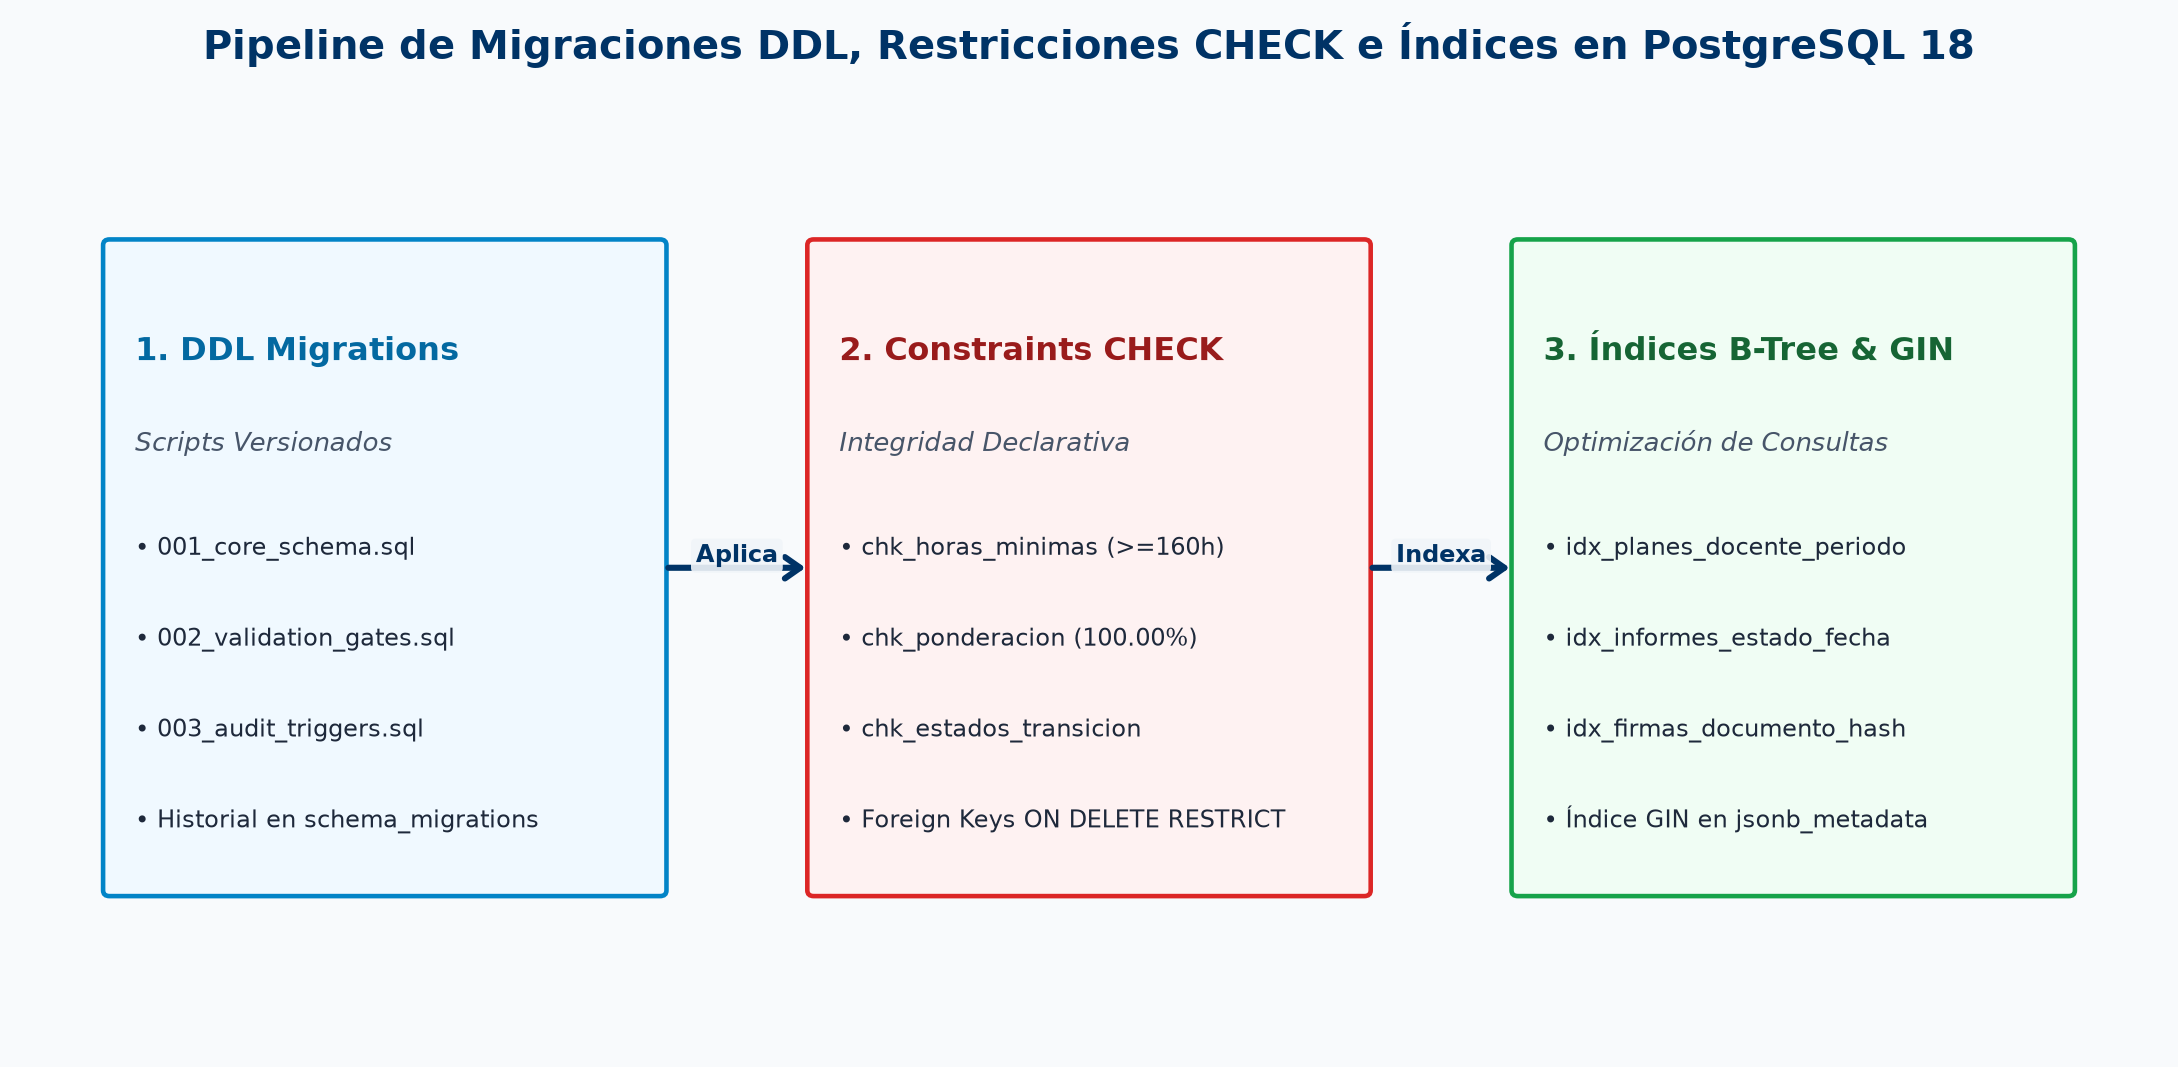
\includegraphics[width=0.88\textwidth,height=5.8cm,keepaspectratio]{images/f3_01_migraciones_indices_bd.png}
    \caption{Arquitectura de Transacciones y Pools de Conexión entre Controladores Express y PostgreSQL.}
    \label{fig:api_transactions}
\end{figure}
\FloatBarrier

\section{Descripción de actividades}
\subsection{Matriz de Endpoints RESTful Implementados}
\begin{table}[H]
\centering
\small
\renewcommand{\arraystretch}{1.2}
\begin{tabularx}{\textwidth}{|c|m{3.5cm}|m{2.5cm}|X|c|}
\hline
\rowcolor{tableheader}
\textbf{Método} & \textbf{Ruta URL Endpoint} & \textbf{Controlador} & \textbf{Carga Útil / Parámetros} & \textbf{Código HTTP} \\
\hline
\texttt{GET} & \texttt{/api/planes} & \texttt{listarPlanes} & Filtros: \texttt{?periodo\_id=\&estado=} & 200 OK \\
\hline
\texttt{POST} & \texttt{/api/planes} & \texttt{crearPlan} & \texttt{\{periodo\_id, carrera\_id, dedicacion\}} & 201 Created \\
\hline
\texttt{GET} & \texttt{/api/planes/:id} & \texttt{obtenerPlan} & Parámetro URL \texttt{id} (UUID) & 200 OK \\
\hline
\texttt{PUT} & \texttt{/api/planes/:id} & \texttt{actualizarPlan} & \texttt{\{horas\_totales, estado\}} & 200 OK \\
\hline
\texttt{GET} & \texttt{/api/secciones/:planId} & \texttt{listarSecciones} & Parámetro URL \texttt{planId} & 200 OK \\
\hline
\texttt{PUT} & \texttt{/api/secciones/batch} & \texttt{actualizarBatch} & \texttt{\{secciones: [\{id, contenido\}]\}} & 200 OK \\
\hline
\end{tabularx}
\caption{Matriz oficial de endpoints RESTful para persistencia.}
\label{tab:endpoints_matrix}
\end{table}

\subsection{Matriz de Manejo Centralizado de Excepciones HTTP}
\begin{table}[H]
\centering
\small
\renewcommand{\arraystretch}{1.2}
\begin{tabularx}{\textwidth}{|c|>{\bfseries}m{3.5cm}|X|c|}
\hline
\rowcolor{tableheader}
\textbf{Código} & \textbf{Tipo de Excepción} & \textbf{Causa y Comportamiento del Middleware} & \textbf{Registro Log} \\
\hline
400 & Bad Request & Parámetros no conformes con esquema de validación. & Warning \\
\hline
401 & Unauthorized & Token JWT ausente, inválido o expirado. & Security Log \\
\hline
404 & Not Found & El plan o sección solicitada no existe en la base de datos. & Info \\
\hline
409 & Conflict & Intento de editar un plan que ya se encuentra en ``Aprobado''. & Audit Warning \\
\hline
500 & Internal Server Error & Falla no controlada; transacción revertida (\texttt{ROLLBACK}). & Error Crítico \\
\hline
\end{tabularx}
\caption{Códigos de excepción y auditoría en la capa de controladores.}
\end{table}

\section{Firmas de Responsabilidad}

\noindent
\renewcommand{\arraystretch}{1.2}
\begin{tabularx}{\textwidth}{|>{\raggedright\arraybackslash}m{2.9cm}|>{\raggedright\arraybackslash}X|>{\centering\arraybackslash}m{4.6cm}|>{\centering\arraybackslash}m{2.3cm}|}
    \hline
    \rowcolor{tableheader}
    \textbf{ACCIÓN} & \textbf{NOMBRE Y CARGO} & \textbf{FIRMA} & \textbf{FECHA} \\
    \hline
    \textbf{Elaborado por:} & Heidi Villavicencio\newline Analista de Calidad / UI-UX & \parbox[c]{4.4cm}{\centering\vspace{4pt}
\includegraphics[height=1.5cm,width=4.0cm,keepaspectratio]{images/firma_heidi.png}\vspace{4pt}} & 22/09/2026 \\
    \hline
    \textbf{Revisado por:} & Steeven Toala\newline Líder de Proyecto / Arquitecto & \parbox[c]{4.4cm}{\centering\vspace{4pt}
\includegraphics[height=1.5cm,width=4.0cm,keepaspectratio]{images/firma_steveen.png}\vspace{4pt}} & 22/09/2026 \\
    \hline
    \textbf{Aprobado por:} & Ing. Paulo Torres, Mg.\newline Docente Evaluador -- Gestión Proyectos & \parbox[c]{4.4cm}{\centering\vspace{8pt}\textbf{\textcolor{gray!80}{\scriptsize [ PENDIENTE DE APROBACIÓN ]}}\vspace{8pt}} & \textbf{\textcolor{gray!90}{Pendiente}} \\
    \hline
\end{tabularx}

\vspace{0.4cm}

\section{Control de Cambios}

\noindent
\renewcommand{\arraystretch}{1.2}
\begin{tabularx}{\textwidth}{|>{\hsize=0.45\hsize\centering\arraybackslash}X|>{\hsize=1.55\hsize\raggedright\arraybackslash}X|>{\hsize=1.2\hsize\raggedright\arraybackslash}X|>{\hsize=0.8\hsize\centering\arraybackslash}X|}
    \hline
    \rowcolor{tableheader}
    \textbf{Versión} & \textbf{Descripción del cambio} & \textbf{Responsable del cambio} & \textbf{Fecha de aprobación} \\
    \hline
    1.0 & Emisión inicial del entregable según EDT del Tablero Trello & Equipo de Proyecto SIGE & 22/09/2026 \\
    \hline
\end{tabularx}

\vspace{0.4cm}

\section{Anexos}

\subsection*{Anexo 1: Ficha Técnica de la Tarea EDT 3.7 en el Tablero Trello}
\begin{table}[H]
\centering
\small
\renewcommand{\arraystretch}{1.2}
\begin{tabularx}{\textwidth}{|>{\bfseries}m{3.5cm}|X|}
\hline
\rowcolor{tableheader}
\textbf{Parámetro EDT} & \textbf{Detalle Oficial del Tablero Trello} \\
\hline
Código de Tarea & EDT 3.7 \\
\hline
Nombre de la Tarjeta & Endpoints de persistencia de secciones y documentos \\
\hline
Fase Correspondiente & FASE 3. IMPLEMENTACIÓN Y DESARROLLO \\
\hline
Período de Ejecución & 18 de septiembre al 22 de septiembre de 2026 (3 días laborables) \\
\hline
Horas Asignadas & 24 horas hombre netas \\
\hline
Responsables Técnicos & Steeven Toala (ST), Nixon Hurtado (NH) \\
\hline
Entregable Oficial & Controladores RESTful Express v5 (\texttt{documentos.controller.js} y \texttt{secciones.controller.js}) \\
\hline
Estado en el Tablero & 100\% Completado y Verificado en Sprint 2 \\
\hline
\end{tabularx}
\caption{Ficha técnica de la tarea EDT 3.7 en el Tablero Trello.}
\end{table}

\subsection*{Anexo 2: Evidencia de Pruebas de Endpoints con Cobertura REST}
\begin{table}[H]
\centering
\footnotesize
\renewcommand{\arraystretch}{1.15}
\begin{tabularx}{\textwidth}{|c|m{2.5cm}|m{3.5cm}|c|c|}
\hline
\rowcolor{tableheader}
\textbf{ID} & \textbf{Endpoint} & \textbf{Condición de Entrada} & \textbf{Latencia} & \textbf{Resultado} \\
\hline
TC-EP01 & \texttt{POST /api/planes} & Payload válido con 40 horas y periodo activo & 24 ms & 201 Created \\
\hline
TC-EP02 & \texttt{GET /api/planes} & Consulta con filtro \texttt{estado=Borrador} & 12 ms & 200 OK (5 registros) \\
\hline
TC-EP03 & \texttt{PUT /secciones/batch} & Actualización simultánea de 4 secciones TipTap & 38 ms & 200 OK (ACID Commit) \\
\hline
TC-EP04 & \texttt{PUT /api/planes/:id} & Edición de plan en estado ``Aprobado HCD'' & 8 ms & 409 Conflict \\
\hline
\end{tabularx}
\caption{Resultados de pruebas automatizadas sobre endpoints RESTful.}
\end{table}

\subsection*{Anexo 3: Trazabilidad en Repositorio Institucional Git}
\begin{itemize}[leftmargin=1.5em, itemsep=2pt]
    \item \textbf{Repositorio:} \texttt{FISEI\_Project / SIGE}
    \item \textbf{Rama de Trabajo:} \texttt{main}
    \item \textbf{Commit de Consolidación:} \texttt{a5190df - feat(api): controladores RESTful para planes y secciones con transacciones ACID}
    \item \textbf{Archivos Afectados:} \texttt{backend/src/modules/documentos/*}, \texttt{backend/src/modules/secciones/*}, \texttt{Entregables\_Latex/Fase\_3/3.7*.tex}
\end{itemize}


\end{document}
